\documentclass[12pt,twoside]{report}
\usepackage[utf8]{inputenc}
\usepackage{graphicx}
\graphicspath{ {images/} }
\usepackage{caption}
\usepackage{subcaption}
\usepackage[a4paper,width=150mm,top=25mm,bottom=25mm,bindingoffset=6mm]{geometry}
\usepackage{fancyhdr}
\pagestyle{fancy}
\fancyhead{}
\fancyhead[RO,LE]{TOWARDS A THREE-BODY PROBLEM}
\fancyfoot{}
\fancyfoot[LE,RO]{\thepage}
\fancyfoot[LO,CE]{Chapter \thechapter}
\fancyfoot[CO,RE]{Sylvance Mbaka}
\renewcommand{\headrulewidth}{0.4pt}
\renewcommand{\footrulewidth}{0.4pt}

\usepackage[style=authoryear,sorting=none]{biblatex}
\addbibresource{references.bib}

\usepackage{color}
\usepackage{listings}
\usepackage{setspace}
\definecolor{Code}{rgb}{0,0,0}
\definecolor{Decorators}{rgb}{0.5,0.5,0.5}
\definecolor{Numbers}{rgb}{0.5,0,0}
\definecolor{MatchingBrackets}{rgb}{0.25,0.5,0.5}
\definecolor{Keywords}{rgb}{0,0,1}
\definecolor{self}{rgb}{0,0,0}
\definecolor{Strings}{rgb}{0,0.63,0}
\definecolor{Comments}{rgb}{0,0.63,1}
\definecolor{Backquotes}{rgb}{0,0,0}
\definecolor{Classname}{rgb}{0,0,0}
\definecolor{FunctionName}{rgb}{0,0,0}
\definecolor{Operators}{rgb}{0,0,0}
\definecolor{Background}{rgb}{0.98,0.98,0.98}
\lstdefinelanguage{Python}{
	numbers=left,
	numberstyle=\footnotesize,
	numbersep=1em,
	xleftmargin=1em,
	framextopmargin=2em,
	framexbottommargin=2em,
	showspaces=false,
	showtabs=false,
	showstringspaces=false,
	frame=l,
	tabsize=4,
	% Basic
	basicstyle=\ttfamily\small\setstretch{1},
	backgroundcolor=\color{Background},
	% Comments
	commentstyle=\color{Comments}\slshape,
	% Strings
	stringstyle=\color{Strings},
	morecomment=[s][\color{Strings}]{"""}{"""},
	morecomment=[s][\color{Strings}]{'''}{'''},
	% keywords
	morekeywords={import,from,class,def,for,while,if,is,in,elif,else,not,and,or,print,break,continue,return,True,False,None,access,as,,del,except,exec,finally,global,import,lambda,pass,print,raise,try,assert},
	keywordstyle={\color{Keywords}\bfseries},
	% additional keywords
	morekeywords={[2]@invariant,pylab,numpy,np,scipy},
	keywordstyle={[2]\color{Decorators}\slshape},
	emph={self},
	emphstyle={\color{self}\slshape},
	%
}

\title{TOWARDS A THREE-BODY PROBLEM}
\author{Sylvance Mbaka}
\date{26th October 2018}

\begin{document}

\begin{titlepage}
    \begin{center}
    	
\includegraphics[width=0.6\textwidth]{logo3}
        \vspace*{1cm}
        
        \huge
        \textbf{TOWARDS A THREE-BODY PROBLEM: SATELLITES AND THE EARTH(KENYA INTO SPACE)}
        
        \vspace{0.5cm}
        
        \vspace{1.5cm}
        
        \Large
        Sylvance Kerandi Mbaka\\
        I44/2503/2014
        
        \vfill
        \large
        \textbf{\textit{A Research Project submitted as part of the requirement for the
        	Degree of Bachelor of Science Astronomy and Astrophysics}}
        
        
        \vspace{0.8cm}
        
        \large
        \textbf{Department of Physics}\\
        \textbf{University of Nairobi}\\
        \vspace{0.5cm}
        \textbf{October, 2018}
        
        
    \end{center}
\end{titlepage}

\thispagestyle{plain}
\begin{center}
    
    \vspace{0.9cm}
    \textbf{Abstract}
\end{center}
The two body problem in physics involves two masses that are bound to each other by gravitation. The problem is to describe all subsequent velocities and positions of the masses given the initial velocity and positions of the two bodies. Two body solutions will help us in predicting the motion of satellites and we will come up with a simulation to predict future movements.

\vspace{0.9cm}
\textbf{Keywords} Two-Body Problem, Satellites, Simulation. 


\chapter*{Declaration}
I  hereby  declare  that  this  research proposal is  my  own work,  and  has  not  been  submitted  at  any  other university  for  purposes  of  examination  or  as  a  research  proposal.  All  sources  used  have  been  acknowledged  by  means  of  proper  references.

\vspace{0.9cm}
\textbf{Sylvance Kerandi Mbaka}\\
\\
Signature: .....................................\\
Date: .............................................\\

This  research  proposal  has  been  submitted  with  the  approval  from  my  supervisor: \\
Dr. Okeyo George Maumba\\
Lecturer, Department of Physics\\
Email: maumba@uonbi.ac.ke\\
University of Nairobi\\
Nairobi, Kenya.\\

\textbf{Dr. Okeyo George Maumba}\\
\\
Signature: .....................................\\
Date: .............................................\\

\chapter*{Dedication}
To my two siblings, mum and dad. To future endeavors.

\chapter*{Acknowledgements}
I want to thank the department of physics for imparting the skills that have led to this project. I would like to thank my supervisor, Dr Maumba, for inspiring me to undertake this line of research. I thank God for everything.

\tableofcontents

\listoffigures

\listoftables

\chapter{Introduction}
\section{Background information}
We are in the 21st century and space travel is all the more a reality now than it was a century prior. There is an expanded requirement for knowledge on how movement outside our earth can be ventured into using safe routes with an exactness that is of the micrometer-scale. To make this possible, researchers have appropriately gathered data of heavenly bodies motions and extraterrestrial environments. With these equations that describe with accuracy the movement of the bodies were derived. Using this information mankind has been able to send vehicles into space. This has prompted space exploration and all the more significantly space correspondence. Space communication involves the satellites that have been sent into space in the endeavor to narrow the communication gap on the earth below. This has brought about application GPS and Satellite correspondence (which includes the exchange of information through satellites and ground stations). In this task we expect to explore on satellite - earth material science by determining conditions that will suitably portray this framework and by making a straightforward model of the same. We will reach determinations on whether Kenya as nation should wander into space by completing a cost assessment and different variables. 

\section{Statement of the problem}
Kenya, like many other countries in Africa,  has not been able to send a satellite into space despite being one of the leading nations in Africa. Kenya is a huge consumer of satellite technology owing to the number of corporations in this country who depend on it to run their activities. But this satellite technology is outsourced. What does Kenya lack that it is not able to send satellites into space?
However, it is only until recently that Kenya was able to send its first pico-satellite into space in a joint venture with Japan. This was done in collaboration with the University of Nairobi. This heralded a new dawn with Kenya having an interest in space.

We are going to look into this matter from an academic angle inquiring the physics involved in the operation of sending a satellite in space and keeping it in space. Due to the scope of this research and the time given, we will focus mainly on the physics of keeping a satellite in orbit. What are the equations involved in keeping a satellite in motion around the planet earth? What is the cost, in monetary terms, involved in keeping a satellite in orbit? Is Kenya able to meet this specifications?

\section{Justification and Significance of the Study}
Kenya is on the verge of constituting a space agency of which the administration of sending satellites into space on behalf of Kenya will be its prerogative. After many years of absence in the space scene will Kenya be able to handle these leap onto new grounds? In this research we will look into answering these questions. 
We will develop a system of equations that will be used to develop simulations that will show that Kenya is better prepared to launch into space. This study will also show what Kenya might expect to incur in terms of the monetary costs on achieving the objective of sending a satellite into space hence avoiding the factor of surprise when Kenya begins to dig deep into the pocket.
\section{Objectives}
\subsection{Main Objective}
To perform a computer model simulation of an isolated Earth-Satellite system based on the two-body problem astrodynamics and compare simulated data with past collected to prove the correctness of the model.
\subsection{Specific Objectives}
1. Review the physics of the two-body problem.\\                                                                                                                                                                       2. Build a computer model for a Earth satellite system in 3-dimensions.\\
3. Apply the model for the Kenyan satellite 1KUNS-PF.
\section{Methodology}
This research will involve deriving equations simplifying the two-body problem which will later be encapsulated in one equation.  This equation will be changed into a computer program that will simulate the interaction between the earth and the satellites that move around it. This simulation will be done in 3 dimensions using Python as it is rich in scientific libraries that will enable the simulation. We will then proceed to determine the accuracy of the model.

\chapter{Literature Review}
\section{Two body problem}
The problem of motion of bodies relative to each other has long been studied. However it's only until recently that researchers have been able to use the full power of computers to research on these problems. In this project we will  leverage on the research that has been done on n-body problems specifically the two-body problems. The two body problem is able to be solved exactly reproducing the Kepler laws.
Johannes Kepler 1571 to 1630 was able to formulate laws that described the data gathered by Tycho Brahe. These laws were largely empirical. Isaac newton who came after him was able to formulate the laws that  govern motion. Joseph lagrange was able to make these equations more detailed. For this project we will focus on the two body problem. The two body problem states that given two bodies with velocities and masses at a given time,t, seperated by a distance, r, find consecutive values for the v and r henceforth.


\chapter{Theoretical Input: Two-Body Problem}
\section{Discussion}
Sending a satellite into space involves a good deal of planning. For the scope we have we will come up with a theory for orbital mechanics. Satellites are acted upon by many forces while in orbit. These forces are; \\
1. The gravitation of the Earth, Fe.\\
2. The gravitational force from the Sun, Fs.\\
3. The gravitation of nearby and large Jupiter, Fj.\\
4. The centripetal force, Fc.\\
5. The frictional force, Ff.\\
6. The gravitation of nearby satellites, Fsat.\\


It can be shown that forces 2-6 are negligible and the dominant force is that of force 1. This makes up an interesting problem which involves two bodies that attract each other due to gravitation. This problem is called the “Two Body Problem” in physics.

The Two-body problem was first described by Sir Isaac Newton in the year . It inquires,  “ given the positions and velocities of two bodies that act on each other by gravity, at a certain point in time, find the equations that describe the subsequent velocities and positions of the bodies.”
These equations have enabled the advent of mankind into outer space and as a result satellite communications. The satellites that orbit the earth are kept in accurate paths by their engineers. This is only achievable by a good understanding and application of the physics involved. For the scope of this project we will go about solving the two body problem only, this is because an introduction of a third body will complicate the system.\\

\vspace{4cm}
\section{Equations that determine satellite location at any given time, t}
\begin{figure}[h]
	\centering
	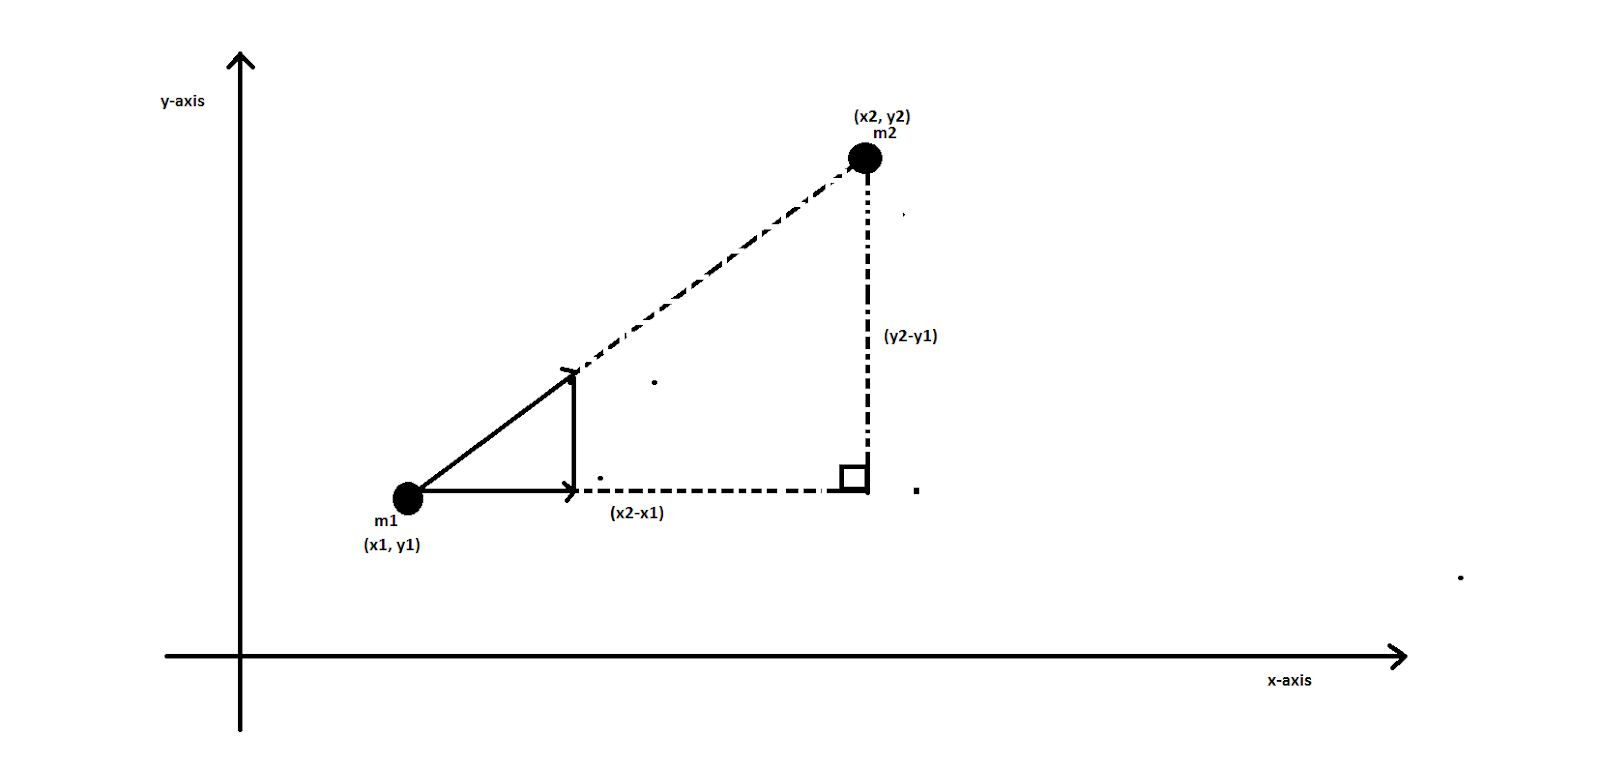
\includegraphics[scale=2.5, width=1\textwidth]{twobody}
	\caption{Two bodies with masses m1 and m2 seperated by a distance r.}
	\label{fig:two-body problem}
\end{figure}
We will now model the two body problem. Let us take a rectangular coordinate frame for the two body problem as shown in the figure above.
\\


The mutual distance apart is r;
\[ r^2 =  (x_2-x_1)^2 + (y_2-y_1)^2  ... \big(1)\]

The magnitude of gravity;
\[ F =  Gm_1m_2 / r^2 ... \big(2)\]
\\
Now the point P1 is attracted to P2 with the force of gravity, F, and can be resolved into the x and y components as;\\
1. along the OX AXIS
\[F_X = Gm_1m_2 / r^2\big(x_2-x_1/r) ... \big(3)\] 
\\
2. along the OY AXIS
\[F_Y = Gm_1m_2 / r^2\big(y_2-y_1/r) ... \big(4)\]
Where, x2-x1/r and y2-y1/r are direct cosines.
\\
For point P2 this will be;\\
1. along the OX AXIS
\[F_X = Gm_1m_2 / r^2\big(x_1-x_2/r) ... \big(5)\] 
\\
2. along the OY AXIS
\[F_Y = Gm_1m_2 / r^2\big(y_1-y_2/r) ... \big(6)\]
Where, x1-x2/r and y1-y2/r are direct cosines.
\\
From Newton’s 2nd Law of motion we have;
\[F=ma\]
\\
We can further work on equations 3) to 6) to obtain the following;\\
1. for particle 1
\[F_X = m_1\big(d^2x/dt^2)= Gm_1m_2 / r^2\big(x_2-x_1/r) ... \big(7)\] 
\[F_Y = m_1\big(d^2y/dt^2)= Gm_1m_2 / r^2\big(y_2-y_1/r) ... \big(8)\]
2. for particle 2
\[F_X = m_2\big(d^2x/dt^2)= Gm_1m_2 / r^2\big(x_1-x_2/r) ... \big(9)\]
\[F_Y = m_2\big(d^2y/dt^2)= Gm_1m_2 / r^2\big(y_1-y_2/r) ... \big(10)\]
\\
Simplifying equations 7) to 10) respectively to obtain equations 11) to 14);\\
1. for particle 1
\[d^2x_1/dt^2= Gm_2 / r^2\big(x_2-x_1/r) ... \big(11)\] 
\[d^2y_1/dt^2= Gm_2 / r^2\big(y_2-y_1/r) ... \big(12)\]
2. for particle 2
\[d^2x_1/dt^2= Gm_1 / r^2\big(x_1-x_2/r) ... \big(13)\]
\[d^2y_1/dt^2= Gm_1 / r^2\big(y_1-y_2/r) ... \big(14)\]
\\
Let us subtract equation 11) from equation 13);
\[\frac{d^2x_2}{dt^2} - \frac{d^2x_1}{dt^2}= \frac{Gm_1} {r^3}\big(\frac{x_1-x_2}{r}) - \frac{Gm_2} {r^3}\big(\frac{x_2-x_1}{r}) ... \big(15)\]

\[\frac{d^2\small(x_2-x_1)}{dt^2}= -\frac{G} {r^3}\bigg[\big(m_1+m_2)-\big(x_2-x_1)\bigg] ... \big(16)\]
Let  \(x = x_2-x_1 ... \big(17)\) and 
\(\mu = G(m1+m2) ... \big(18)\) 
then;
\[\frac{d^2x}{dt^2}+\frac{\mu x}{r^3}=0 ... \big(19)\]
\\
In a similar fashion for equations 12) and 14) we arrive at;
\[\frac{d^2y}{dt^2}+\frac{\mu y}{r^3}=0 ... \big(20)\]
where;
\[y = y_2-y_1 ... \big(21)\]

The solution of this is written as;
\[r = \frac{\frac{h^2}{\mu}}{1+e\cos\theta} ... \big(22)\]

where \(\theta\) is the true anomaly, h is a constant which is twice the rate of description of area by radius vector, e, is the eccentricity of the orbit.\\

To prove this, consider; 
\[r^2 = \big(x_2-x_1)^2+\big(y_2-y_1)^2 ... \big(23)\]
equation 15) and 16) can be combined as; 
\[\frac{d^2r}{dt^2}+\frac{\mu\vec{r}}{r^3}=0 ... \big(24)\]
\[\ddot{\vec{r}}+\frac{\mu\vec{r}}{r^3}=0 ... \big(25)\]
\[\ddot{\vec{r}}=-\frac{\mu\vec{r}}{r^3} ... \big(26)\]\\
crossing both side with \(\vec{r}\) we will have;
\[\vec{r}\times\ddot{\vec{r}}=-\vec{r}\times\frac{\mu\vec{r}}{r^3}\]
\[=0 ... \big(27)\]\\
the left hand side can be written as;
\[\vec{r}\times\ddot{\vec{r}}= \frac{d}{dt}\big(\vec{r}\times\dot{\vec{r}}) ... \big(28)\]\\
since the time derivative of \(\vec{r}\times\dot{\vec{r}}\) is equal to zero, the quantity itself must be a constant, i.e.; \(\vec{r}\times\dot{\vec{r}}=\vec{h}=constant\).\\
The vector \(\vec{h}\) is the angular momentum per unit mass. It is related to the angular momentum vector \(\vec{l}\) by;
\[\vec{l}= m\vec{h}\]
where \(m\) is the mass of the particle.\\

Considering by Kepler's second law, then the motion of this particle over a small time step \(\Delta t\), we have;
\[\Delta A = \frac{1}{2}\arrowvert r\times \dot{r}\Delta t\arrowvert ... \big(29)\]
\[=\frac{1}{2}\arrowvert\vec{h}\arrowvert\Delta t ... \big(30)\]

Therefore;
\[\vec{h}\times\ddot{\vec{r}}=-\frac{\mu\big(\vec{h}\times\vec{r})}{r^3}  ... \big(31)\]
\[=-\frac{\mu}{r^3}\big[\big(\vec{r}\times\dot{\vec{r}})\times\vec{r}  ... \big(32)\]
\[=-\frac{\mu}{r^3}\big[\dot{\vec{r}}\big(\vec{r}\cdot\vec{r})-\vec{r}\big(\vec{r}\cdot\vec{r})]  ... \big(33)\]

now since;
\[\frac{d}{dt}\bigg(\frac{\vec{r}}{r}\bigg)=\frac{1}{r}\dot{r}-\frac{\dot{r}}{r^2}\vec{r}  ... \big(34)\]
\[=\frac{1}{r^3}\big[\dot{\vec{r}}\big(\vec{r}\cdot\vec{r})-\vec{r}\big(\vec{r}\cdot\dot{\vec{r}})]  ... \big(35)\] 

then;
\[\vec{h}\times\dot{r}=-\mu\frac{d}{dt}\bigg(\frac{\vec{r}}{r}\bigg)  ... \big(36)\]

integrating both sides with respect to time will yield;
\[\vec{h}\times\dot{r}= -\mu \frac{\vec{r}}{r}- \vec{A}  ... \big(37)\]

where A is determined by the initial position and velocity.\\

We multiply through by \(\vec{r}\);
\[\big(\vec{h}\times\dot{r})\times\cdot\vec{r}= -\mu \boldmath{r}- \vec{A}\cdot\vec{r}  ... \big(38)\]

If we introduce, \(\nu\), as the true anomaly, the angle between A and the position vector \(\vec{r}\), we obtain;
\[h^2=\mu r + Ar \cos \nu  ... \big(39)\]
since
\[\big(a\times b\big)\cdot c = -\big(c\times b\big)\cdot a  ... \big(40)\]
letting \(P=h^2/\mu \) and \(e = A/\mu \) then;
\[r=\frac{P}{1+e \cos \nu}  ... \big(41)\]
For the above equation for any conic section except a parabola we will have
\[P = a\big(1-e^2)   ... \big(42)\]

therefore;
\[r=\frac{a\big(1-e^2)}{1+e \cos \nu}   ... \big(43)\]

Now we will use this equation to get the position of the satellite in it's orbit from the central body. We still have the problem which is described as; what is the position of a satellite in it's orbit after an elapsed time, \(t-t_o\). We can further refine the problem as; how long does it take for the satellite to move from one point to another in its orbit.

Kepler was able to solve this problem by defining the Mean Anomaly, the part of the orbit form the centre which the satellites sweeps relative to the perigee. Perigee is the shortest point to the centre along the satellite's orbit. 

The change in Mean Anomaly is defined as;
\[M-M_o = n(t-t_o)   ... \big(44)\]

where;
\[n=\sqrt{\frac{\mu}{a^3}}   ... \big(45)\] 

We define a variable \(E\) called the eccentric anomaly which can be written as;
\[cos E = \frac{ae + r \cos \nu}{a}   ... \big(46)\]
\[ \cos E = \frac{e+\cos \nu}{1+e \cos \nu}   ... \big(47)\]

given the above we will have the mean anomaly as;
\[M= E-sinE   ... \big(48)\]
this is Kepler's equation.



\chapter{Methodology}
\section{Simulation preparation}
Now that we have the equations that govern the motion of a satellite in place we can proceed to write a computer program that will simulate the trajectory a satellite takes after it is put in orbit. When a satellite is placed in its orbit it will have values of \(r\) and \(\nu\) change as time goes by. This coupled with inclination of the orbit will aid in locating the position of the satellite in its orbit.

The diagram below illustrates the elements used to locate a satellite in its orbit;
\begin{figure}[h]
	\centering
	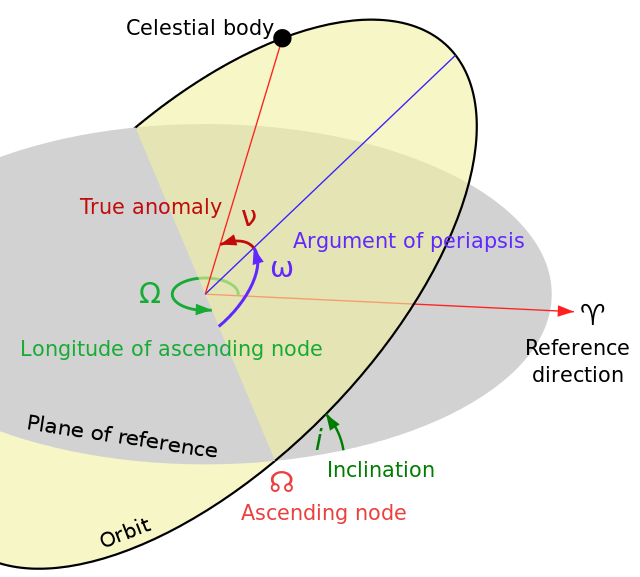
\includegraphics[width=0.4\textwidth]{orbit}
	\caption{Orbital elements for a satellite.}
	\label{fig:six-orbital-elements}
\end{figure}

\subsection{Satellite launch data acquisition}
For each satellite launched into space the data of it's launch variables are provided by NASA and can be acquired from \textcite{http://celestrak.com}. Of particular interest is the Kenyan satellite launched into space in the year 2018. The particular launch data is at \textcite{http://celestrak.com/satcat/tle.php?CATNR=43467}. This will give us a two-line-element from which we will extract the particular values for the satellite of interest.

From the Two-Line-Element we will be able to deduce the orbital elements of 1KUNS-PF namely its eccentricity, mean anomaly, mean motion and the Argument of Perigee.


The Two-Line-Element for 1KUNS-PF is this;\\
\textcite{1KUNS-PF}\\              
\textcite{1 43467U 98067NQ  18290.48306199  .00009882  00000-0  13782-3 0  9995}\\
\textcite{2 43467  51.6385 126.6004 0002599 213.4711 146.6117 15.57589009 24750}\\

From this we are able to define inclination=51.6385, eccentricity=0.002599, mean anomaly=146.6117, mean motion=15.57589009 and the Argument of Perigee=213.4711.

We will use this values to write a computer program that will simulate the trajectory that 1KUNS-PF will follow.

We also use celestrak to acquire more data for cubesats that were launched in 2018. This data will be used to simulate multiple satellites orbiting the earth.

\subsection{Position Simulation Algorithmn}
The algorithmn we will use to determine the position of the satellite;\\
\begin{description}
	\item[1.] Set the values that define the satellite orbit.
	\item[2.] Set the time to the required start position and set the time step for simulation.
	\item[3.] Get the initial values for the orbital elements for the satellite.
	\item[4.] Convert these values from polar coordinates to cartesian coordinates.
	\item[5.] Plot the cartesian values in a 3 dimensional graph.
	\item[6.] Plot the orbit for the satellite.
	\item[7.] Plot the earth in 3 dimensions using the standard lengths.
	\item[8.] Increment the time step.
	\item[9.] Repeat step 1-8 with updated values for the satellite position.
\end{description}

The code that implements this algorithmn has been further discussed in the appendix in much detail. The language of choice used in this simulation is Python as it is rich with scientific tools, has a good community and fully-fledged libraries. Matplotlib, numpy and jupyter notebook were employed in the creation of these simulations.

Numpy has been used to work the numbers into a suitable format to work with. Matplotlib has been used for the plotting and simulation itself. Jupyter was used for development purposes.
\subsection{Time step}
For this particular case we will use the default timestep provided by matplotlib FuncAnimation library. This will ensure that we only get to worry about the position itself and not how the display of the animation works.
\\
\\
\\
\section{Simulation}
\subsection{Dummy satellite simulation}
The simulation was done for a dummy satellite as shown below;
\begin{figure}[h]
	\centering
	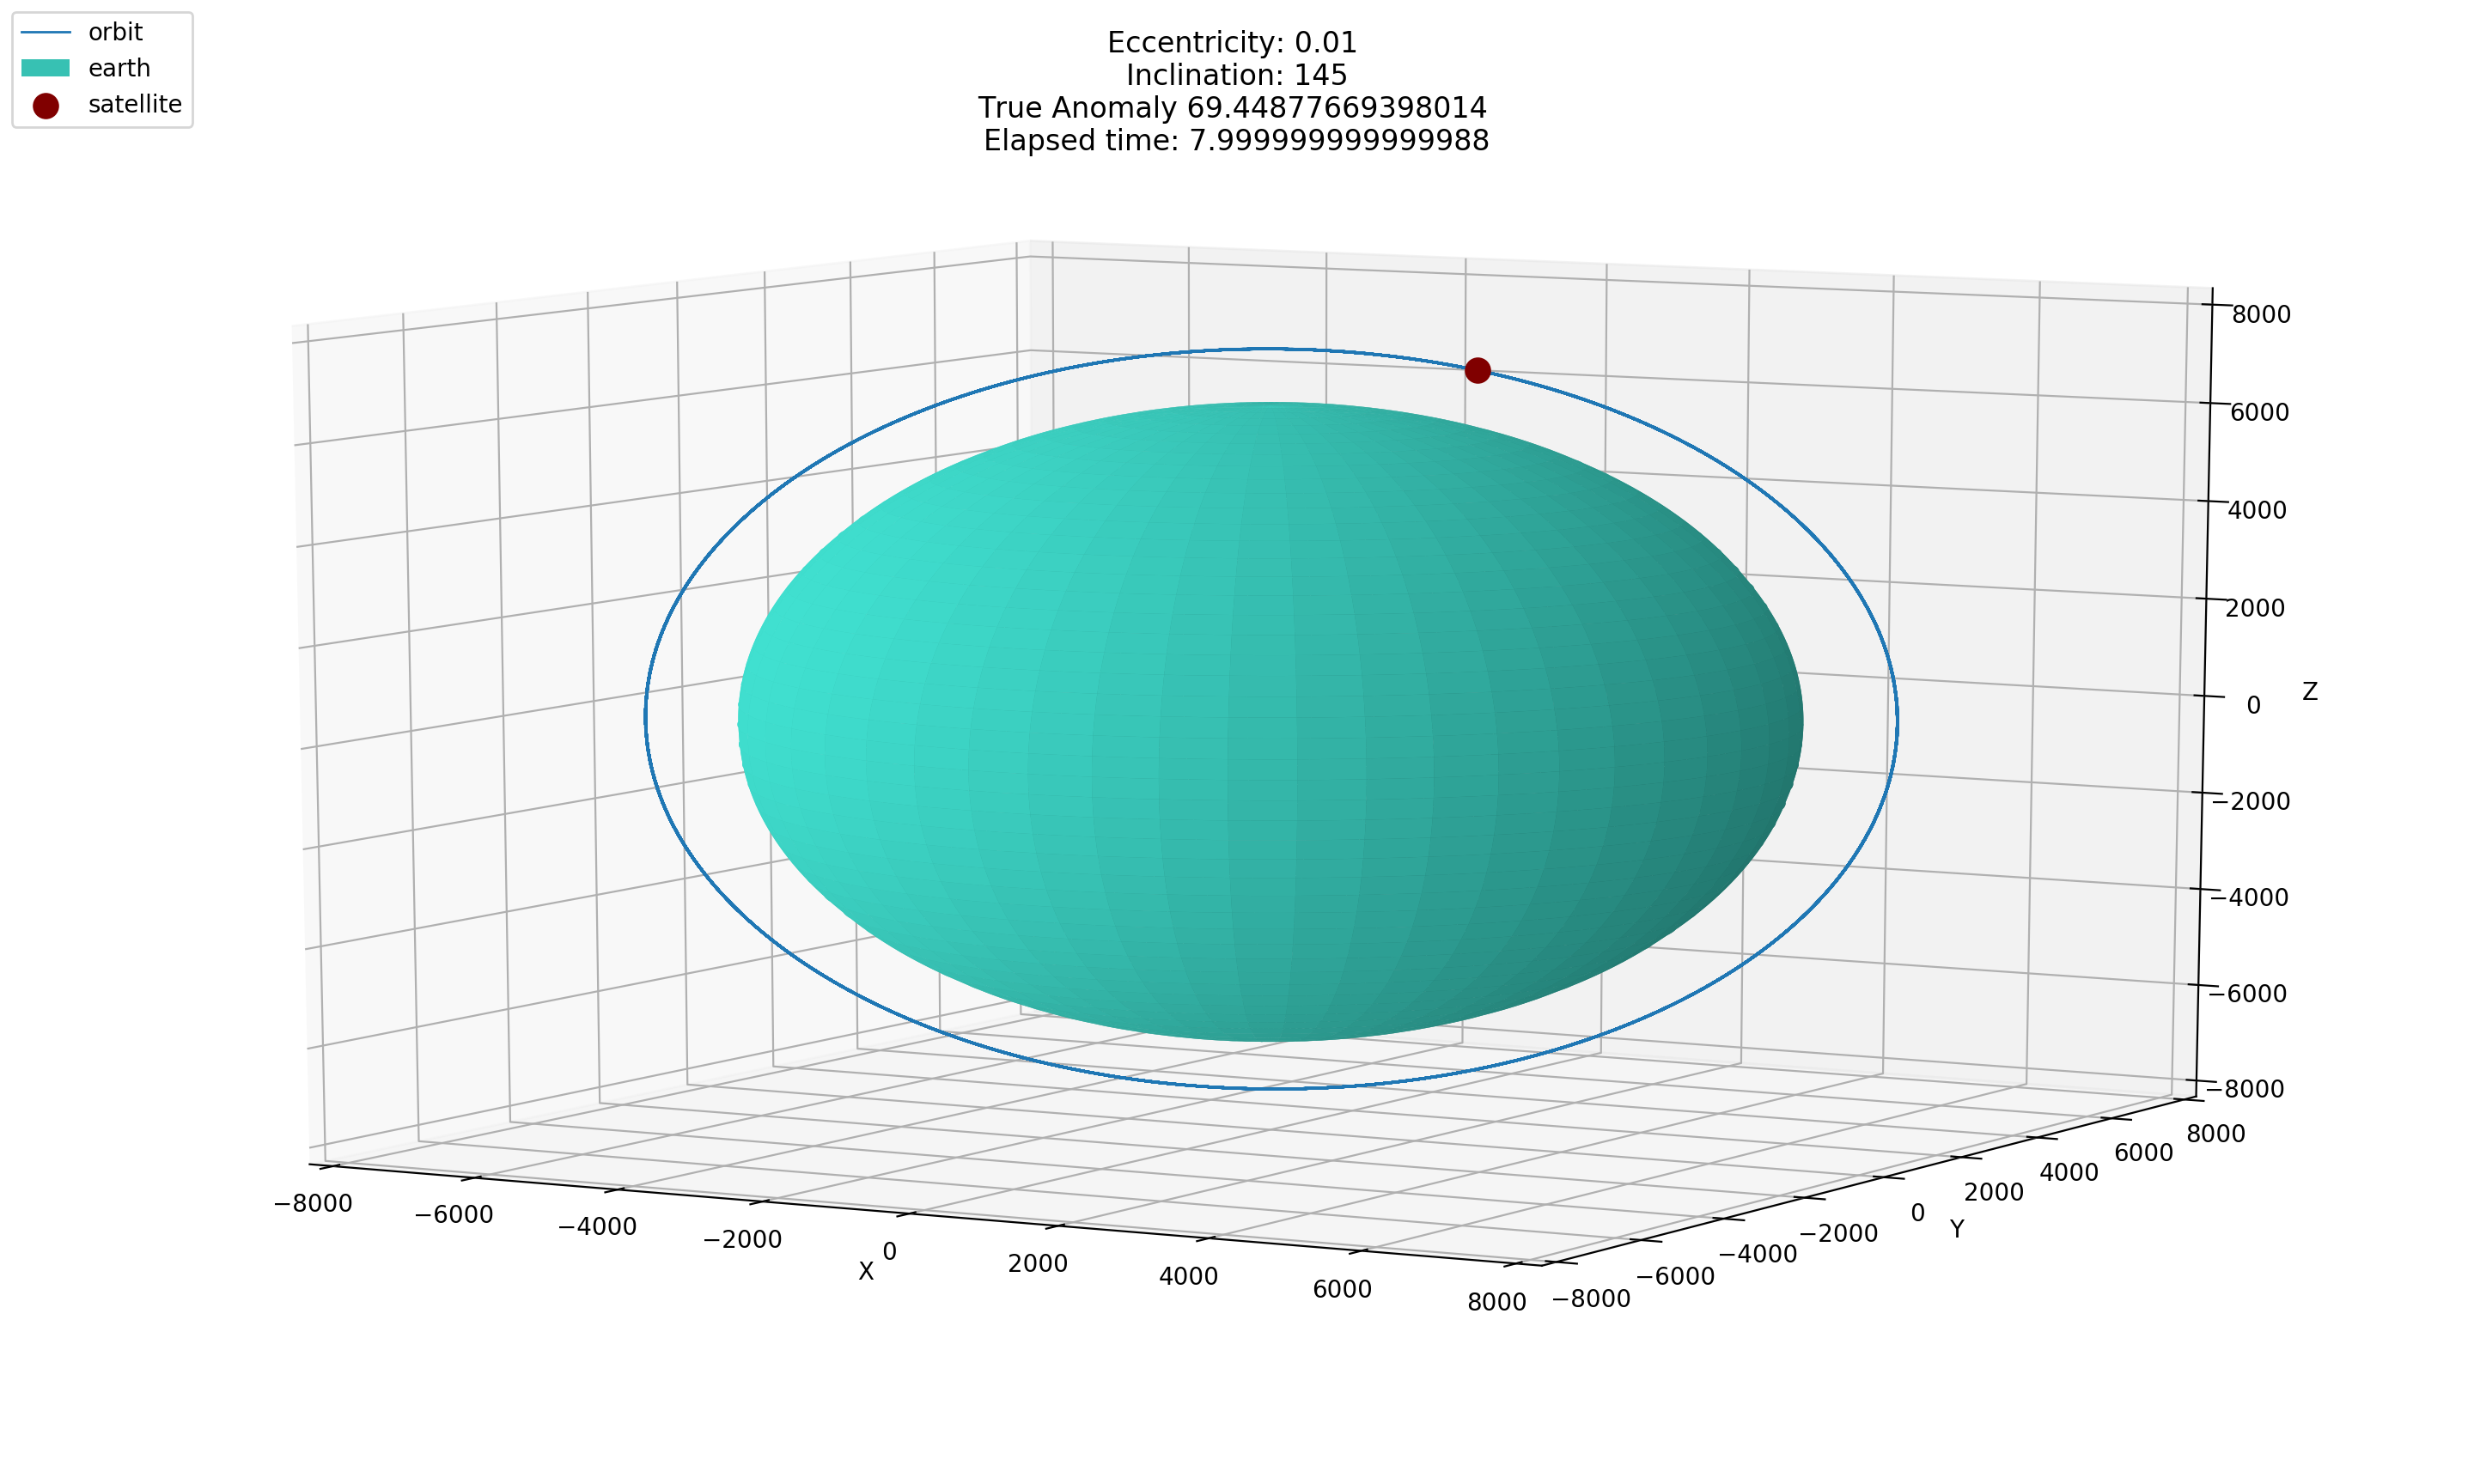
\includegraphics[width=1.2\textwidth]{3d_satellite}
	\caption{Dummy satellite: elev=10., azim=-60.}
	\label{fig:dummy-satellite}
\end{figure}

The values used for this satellite were; dummy-sat = Satellite(1, 0.01, 7500, 145, 69)   where Satellite(mass, eccentricity, semi-major-axis, inclination, true-anomaly) is the python class that defines the satellite.

The satellite is moving in a medium earth orbit \textbf{LEO} with a retrogade motion\big(moving in a different direction as the rotation of the earth). The altitude of the satellite of the satellite at perigee is 1046.85km.

\subsection{1KUNS-PF satellite simulation}
The simulation was done for 1KUNS-PF satellite, with semi-major axis being 6778.8km, as shown below in Figure 4.3.
\begin{figure}[h]
	\centering
	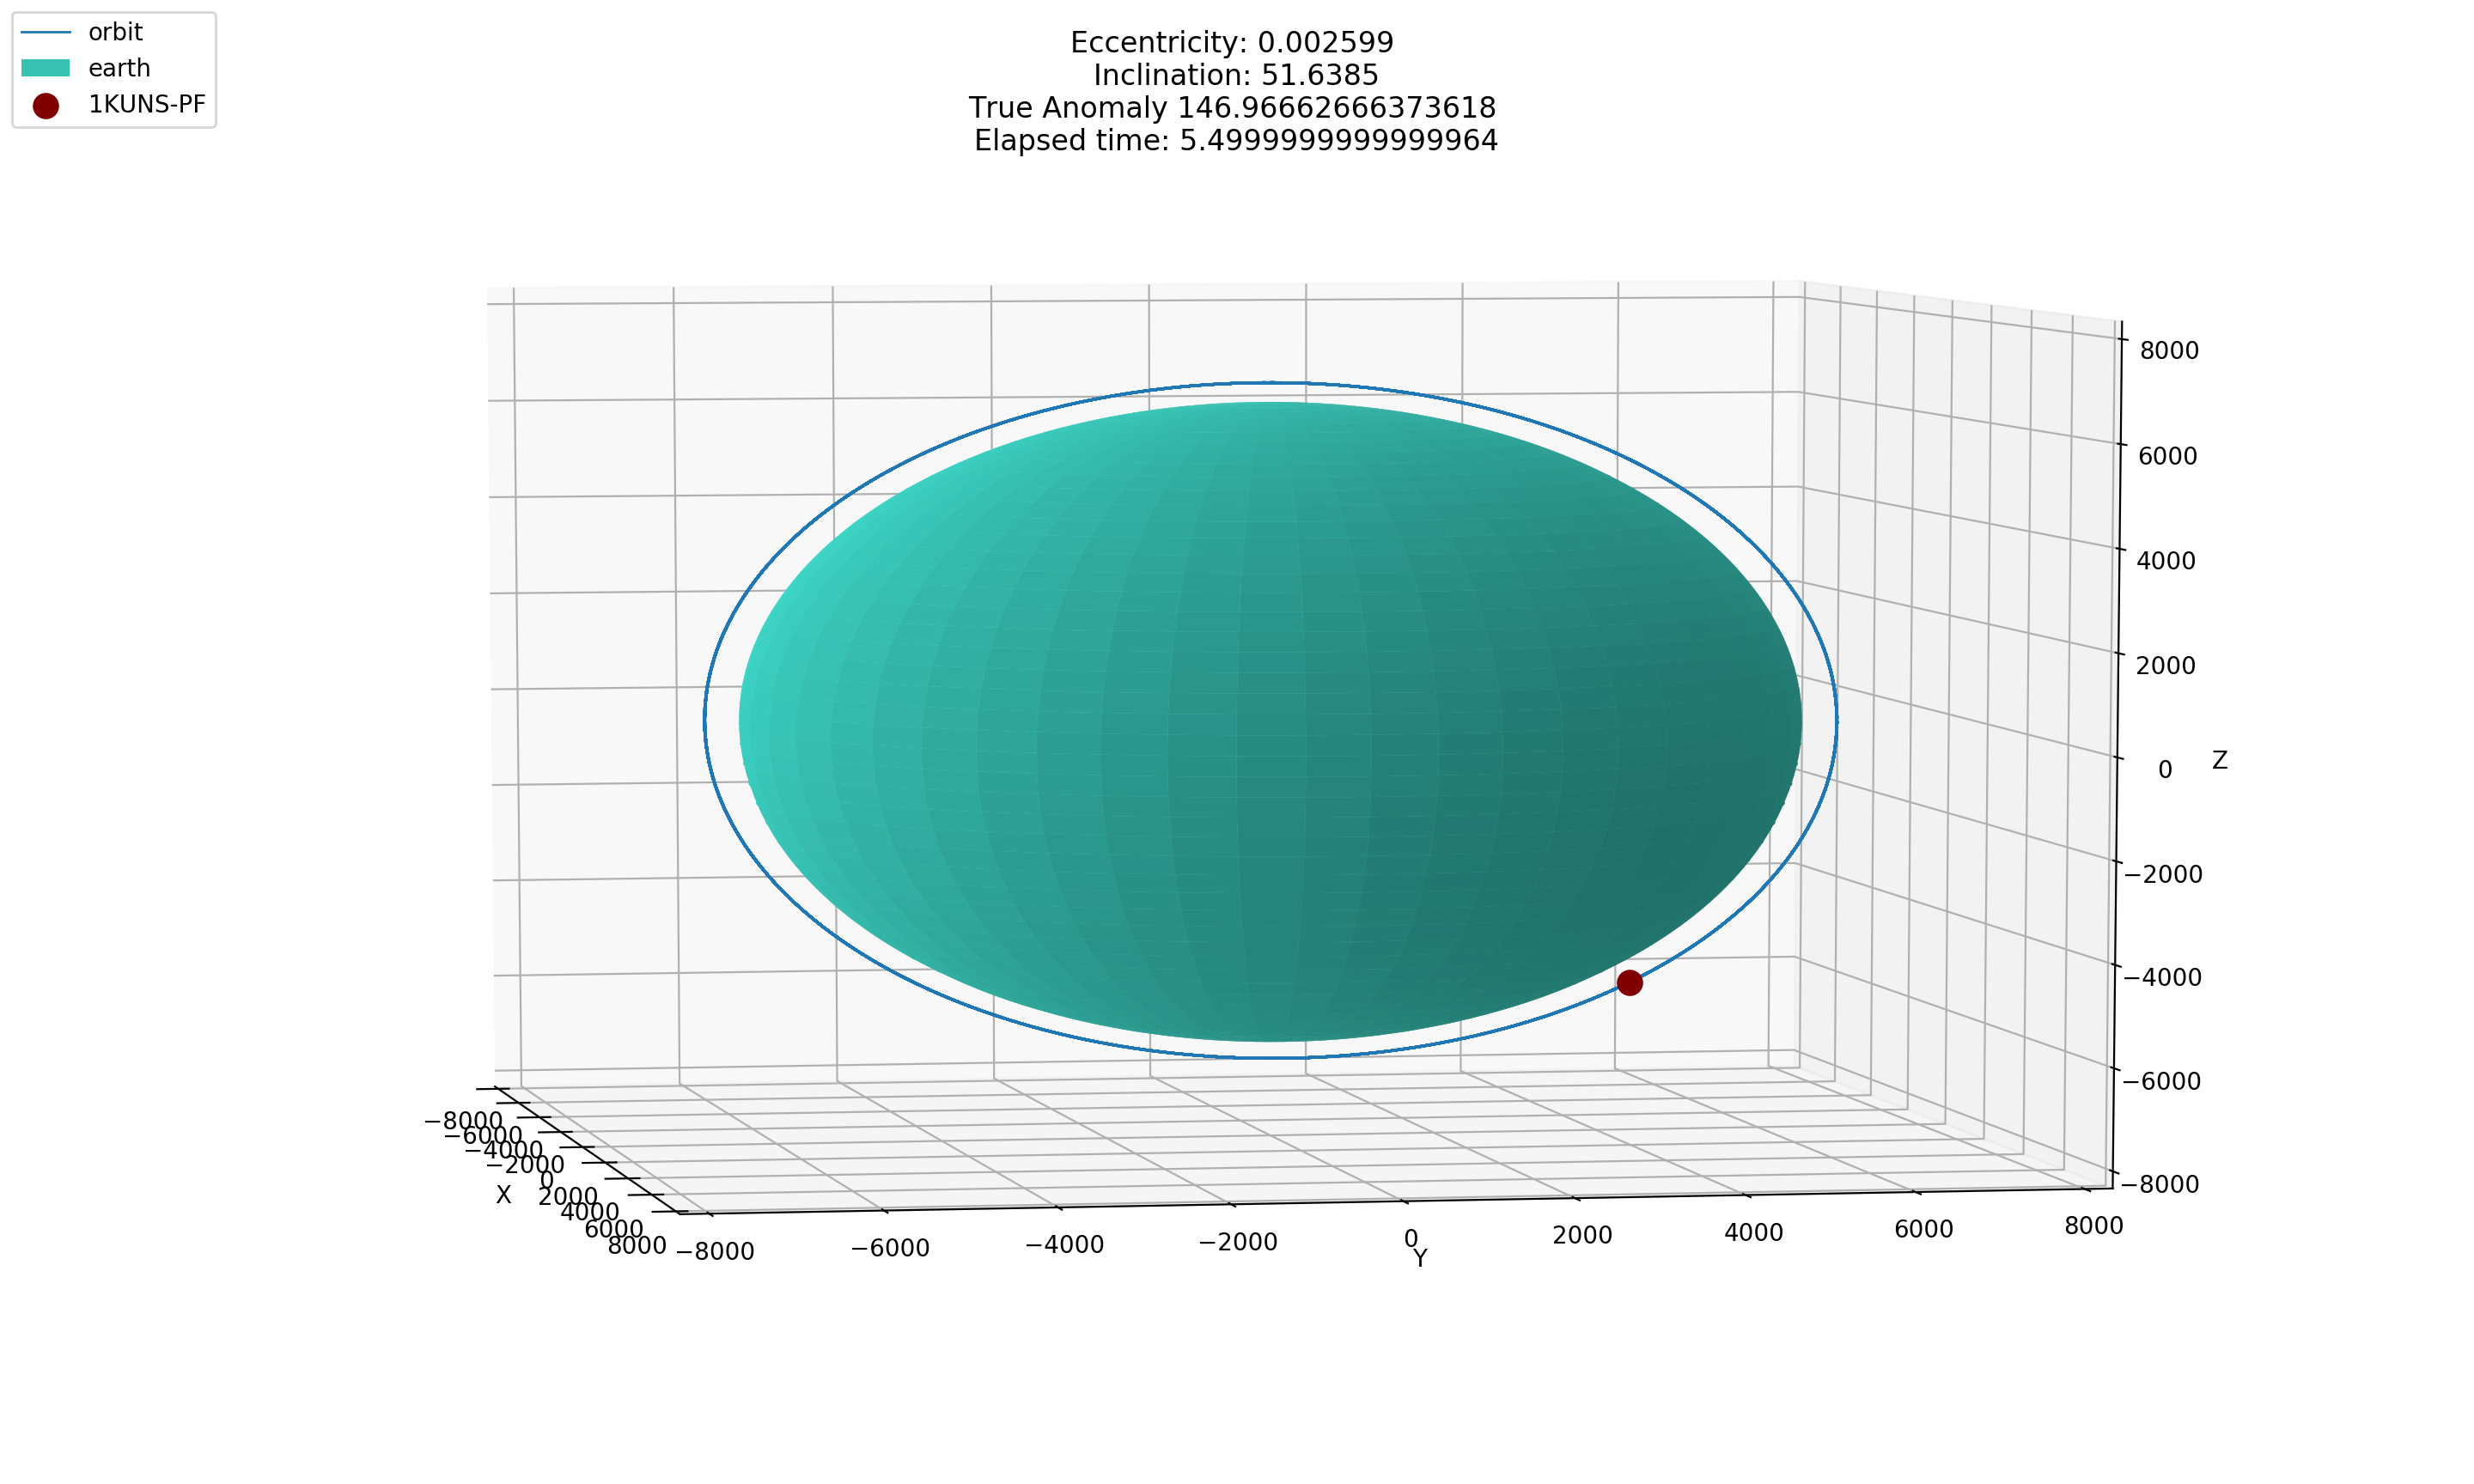
\includegraphics[width=1.2\textwidth]{1kuns-pf}
	\caption{1KUNS-PF: elev=-10., azim=5.}
	\label{fig:1KUNS-PF}
\end{figure}

The values used for this satellite were; kuns = Satellite(1, 0.002599, 6778.8, 51.6385, 146.6117)   where Satellite(mass, eccentricity, semi-major-axis, inclination, true-anomaly) is the python class that defines the satellite.

The satellite is moving in a low earth orbit \textbf{LEO} with a posgrade motion, moving in the same direction as the rotation of the earth. The altitude of the satellite of the satellite at perigee is 383.04km. This is quite close as compared with the actual figure which 398.9 km according to 
\textbf{https://www.n2yo.com/satellite/?s=43466}.
\subsection{3-Body simulation: 1KUNS-PF and Dummy-Sat satellite simulation}
The simulation was done for 1KUNS-PF satellite and the dummy sat as shown in Figure 4.4. The values used for this satellite were; kuns = Satellite(1, 0.002599, 6778.8, 51.6385, 146.6117)  and dummy-sat = Satellite(1, 0.01, 7500, 145, 69) where Satellite(mass, eccentricity, semi-major-axis, inclination, true-anomaly) is the python class that defines the satellite.

For this case we have use matplolib's plot-wireframe method to represent the earth in 3-d dimensions.

In this case we define \(r_{kuns}\) and \(r_{dummy}\) for 1KUNS-PF and dummy-sat respectively as;
\[r_{kuns}=\frac{a_{kuns}\big(1-e_{kuns}^2)}{1+e_{kuns} \cos \nu_{kuns}} \]
\[r_{dummy}=\frac{a_{dummy}\big(1-e_{dummy}^2)}{1+e_{dummy} \cos \nu_{dummy}} \]

This will give a wireframe figure as an attempt towards simulation of the three body-problem.
\begin{figure}[h]
	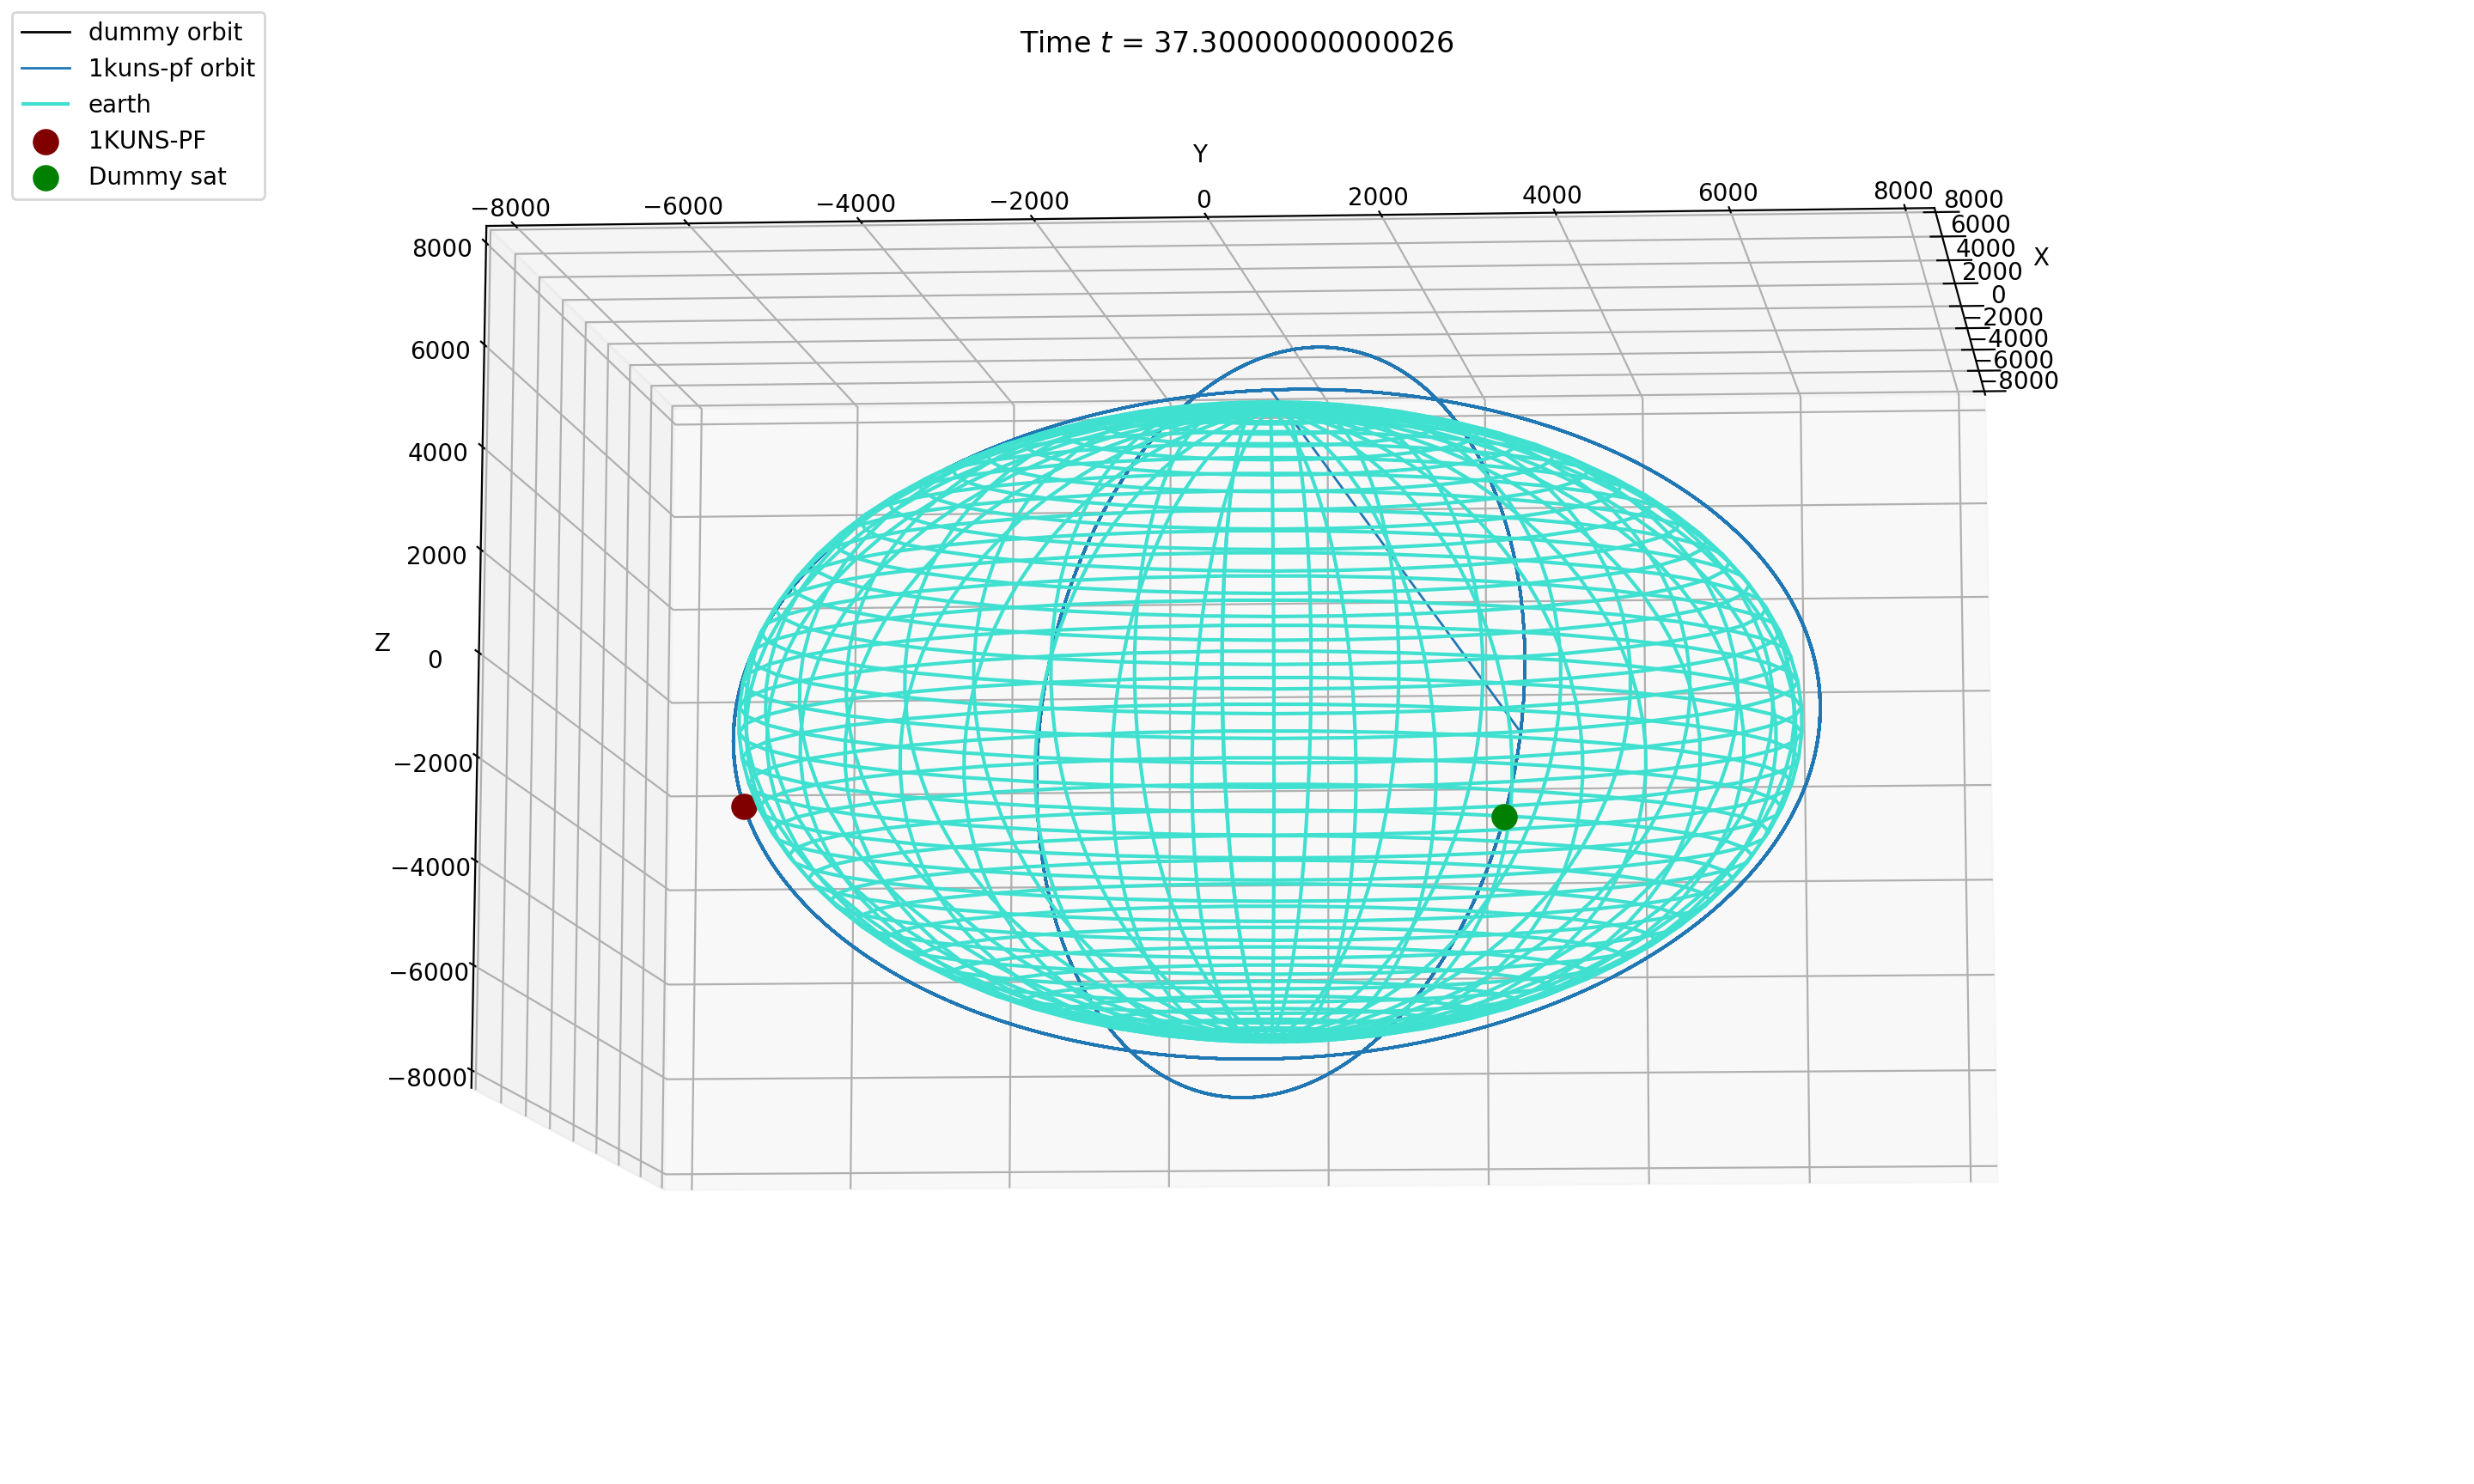
\includegraphics[width=1.2\textwidth]{3body}
	\caption{3-body simulation: 1KUNS-PF and Dummy-sat elev=-10., azim=5.}
	\label{fig:3body-sim}
\end{figure}	






\chapter{Results and Discussion}
\section{Simulation KUNS-DATA}
\begin{tabular}{ |p{4cm}|p{4cm}|p{4cm}|p{4cm}|  }
	\hline
	\multicolumn{4}{|c|}{1KUNS-PF SATELLITE: Initial 32 steps} \\
	\hline
	X-coordinate& Y-coordinate & Z-coordinate & r-value \\
	\hline
	0.0 & 0.0 & 7499.26 & 7499.26 \\
	661.7279520047292 & 350.189924537281 & 7461.794886794123 & 7499.259950041653\\
	1316.8441108213185 & 696.8808532249893 & 7349.773889180901 & 7499.259800665778\\
	1958.8027471592993 & 1036.6087515768586 & 7164.316292753275 & 7499.259553364891\\
	2581.189599393226 & 1365.979158488787 & 6907.275142809683 & 7499.25921060994\\
	3177.7859636668654 & 1681.7011030602155 & 6581.218728767907 & 7499.258775825619\\
	3742.63082993031 & 1980.619987312898 & 6189.404921900176 & 7499.258253356149\\
	4270.080443035229 & 2259.7491062368476 & 5735.7486228289135 & 7499.257648421873\\
	4754.864693747449 & 2516.299490211804 & 5224.782644074119 & 7499.256967067094\\
	5192.139776217474 & 2747.7077716185368 & 4661.612418543307 & 7499.256216099683\\
	5577.536585761735 & 2951.6617972001086 & 4051.8649865474645 & 7499.2554030230585\\
	5907.20437337694 & 3126.1237302612585 & 3401.632771095174 & 7499.254535961214\\
	6177.849220811461 & 3269.350411879238 & 2717.4127032906154 & 7499.253623577545\\
	6386.766951777119 & 3379.910777690777 & 2006.0413061191698 & 7499.252674988286\\
	6531.87015048454 & 3456.700156243592 & 1274.6263852829277 & 7499.251699671429\\
	6611.709017569755 & 3498.951306062806 & 530.476009644038 & 7499.250707372016\\
	6625.485855060067 & 3506.242081171336 & -218.97450909181913 & 7499.249708004777\\
	6573.063035688075 & 3478.499648492932 & -966.2369078366777 & 7499.248711555057\\
	6454.964376967799 & 3416.001215020513 & -1703.844792419215 & 7499.247727979053\\
	6272.369906345426 & 3319.3712575063164 & -2424.4282391396887 & 7499.246767104331\\
	6027.104069770971 & 3189.5752823757875 & -3120.7874321942622 & 7499.245838531635\\
	5721.617501546105 & 3027.9101782348425 & -3785.964601224588 & 7499.244951538954\\
	5358.962537633365 & 2835.9912573838687 & -4413.313540241502 & 7499.244114988827\\
	4942.762717120081 & 2615.736115831475 & -4996.5660133453575 & 7499.243337239787\\
	4477.176576592361 & 2369.34547308613 & -5529.89438377777 & 7499.2426260628445\\
	3966.856099190628 & 2099.2811831770573 & -6007.969840579415 & 7499.241988563845\\
	3416.900233518795 & 1808.2416366156667 & -6426.015641118722 & 7499.241431112467\\
	2832.8039468313227 & 1499.1347990732647 & -6779.854837557066 & 7499.24095927858\\
	2220.4033215340437 & 1175.0491561595359 & -7065.952010430044 & 7499.240577776593\\
	1585.817243560537 & 839.2228546035708 & -7281.448592400483 & 7499.240290418348\\
	\hline
\end{tabular}
\captionof{table}{1KUNS-PF Orbit simulations results-32 steps}\label{tbl:kunstable}

\section{Discussion}
The simulation successfully predicted the position of the cubesat with an accuracy of 12 decimal places. This is largely determined by the short timestep chosen of \(0.1 seconds\). This is sufficient time that can be translated to any situation where orbit determination is required.

\section{Software technical debt}
The program is simple to build and does not require alot of infrastructure to implement. It is easily accessible and can be used for research purposes within the university. The software will be hosted online for future purposes of learning and improvement.





\chapter{Recommendations and Conclusions}
\section{Recommendations}
\subsection{Ground-track}
This simulation has not been able to show the ground-track the satellite goes through. As a future improvement this simulation should be able to show the trace that a satellite has on the ground.
\subsection{Earth's rotation}
This simulation has not been able to show the rotation of the earth as the satellite moves around the earth. However, this does not reduce the accuracy of the program in determining the satellites position along it orbit rather it decreases the ability to trace the ground track of the satellite. As a future improvement this simulation should be able to show the earth moving about its axis.

\subsection{Pertubations}
This simulation has not been able to show the effects of perturbations mentioned earlier on the satellite's position along its orbit. This can be done by deriving equations that govern perturbations on the satellite. As a future improvement this simulation should be able to show the effects of perturbations on the satellites motion.

\subsection{Realtime location}
As a future improvement this simulation should be able to locate the subject satellite in realtime. It was not possible for this case because of the recommendations mentioned above. Ideally, one should be able to determine the ground track to successfully for one to locate the satellite correctly.

\subsection{Conclusions}
The objectives of this project were fully met as we were able to simulate the satellite's motion of 1KUNS-PF in 3 dimensions. The accuracy of up to 12 decimal places was satisfactory.

Future improvements can be made to make the program more accurate and include many bodies to the simulation.

\begin{thebibliography}{1}
	
	\bibitem{bib1}
	Peter Fortescue, John Stark, Graham Swinerd.
	\newblock {\em \mbox{Spacecrafts Engineering Systems} }, Wiley, 2003.
	
	\bibitem{bib2}
	Aamport.Oliver Montenbruck, Eberhard Gill.
	\newblock {\em \mbox{Satellite Orbits} }, Springer, 2001.
	
	\bibitem{bib3}
	Roger R. Bate, Donald D. Mueller, Jerry E. White.
	\newblock {\em \mbox{Fundamentals of Astrodynamics}  }, Dover, 1971.
	
	\bibitem{bib4}
	Jon Toellner.
	\newblock \(https://www.youtube.com/watch?v=U_KJtzJl5_c \),\\
	\newblock {\em \mbox{Orbital Dynamics The Two Body Problem}}, Youtube, 2018.
	
	\bibitem{bib5}
	Brittanica of Science.
	\newblock \(www.britannica.com/science/celestial-mechanics-physics\),
	\newblock {\em \mbox{Celestial Mechanics Physics}}, Brittanica of Science, 2018.    
	
	
\end{thebibliography}

\appendix
\chapter{Appendix Title}
The code for this simulation is as shown below. For easier reading only the code for the three-body simulation has been included as it contains code for the previous 2 simulations;

\section{Code}
\lstinputlisting[language=Python]{sim3d-animated.py}

\end{document}
